\section{Higher-degree Polynomials}

    \subsection{Graphing Higher-degree Polynomials}
        \color{purple} \textbf{Steps to Graph Higher-Degree Polynomials:} \color{black} \\

        \noindent 1. Determine the zeroes of the polynomial $P(x)$ and their multiplicity. \\
        2. Determine the $y$-intercept, $(0, P(0))$ \\
        3. Use the Leading Coefficient Test to determine the end behaviors. \\
        4. Plot a few more points to make the sketch more accurate.
        At least plot one point at each end and between each of the zeroes. \\

        \noindent The first three names of higher-degree polynomials are \textbf{cubic} ($x^3$),
        quartic ($x^4$), and quintic ($x^5$). Polynomials that are second-degree and higher
        tend to be \textit{continuous} and there are usually local maxima and minima. \\

        \noindent A polynomial with degree $n$ will have at most $n-1$ extrema. \\

        \noindent \color{purple} \textbf{The Multiplicity Test}: \\

        \noindent \color{black}
        If $x=r$ is a zero of the polynomial $P(x)$ with multiplicity $k$ then:  \\
        1. If $k$ is odd then the $x$-intercept corresponding to $x=r$ will cross the x-axis. \\
        2. If $k$ is even then the $x$-intercept corresponding to $x=r$ will only touch the
        x-axis and not cross it. \\

        \noindent Furthermore, if $k>1$ then the graph will flatten out at $x=r$. \\

        \noindent \color{purple} \textbf{Multiplicity} \color{black} refers to the number of
        times a factor is found within a polynomial. Consider the polynomial given by
        $P(x)=x^2(x-3)(x+2)$. Its zeroes are $x=-2$ ($k=1$), $x=0$ ($k=2$), and
        $x=3$ ($k=1$). $x=0$ has a mutliplicity of 2, since the factor appears twice.
        Recall that $x^2=0$ gives $x=\pm 0$. \\

        \noindent \color{purple} \textbf{The Leading Coefficient Test:} \color{black} Suppose
        that $P(x)$ is a polynomial with degree $n$, where $P(x)=ax^n+\dots$. We only need to
        consider the first coefficient, $a$. \\

        \noindent 1. If \textbf{$a>0$ and $n$ is even} then the graph of $P(x)$ will increase without
        bound at both endpoints. \\
        \begin{figure} [hbt!]
            \centering
            \includegraphics[scale = 0.5] {Resources/Unit4HigherPolynomials/leadcoeff1.png}
        \end{figure}

        \noindent 2. If \textbf{$a>0$ and $n$ is odd} then the graph of $P(x)$ will increase without bound
        at the right end and decrease without bound at the left end. \\
        \begin{figure} [hbt!]
            \centering
            \includegraphics[scale = 0.5] {Resources/Unit4HigherPolynomials/leadcoeff2.png}
        \end{figure}

        \noindent 3. If \textbf{$a<0$ and $n$ is even} then the graph of $P(x)$ will decrease without
        bound on both ends. \\
        \begin{figure} [hbt!]
            \centering
            \includegraphics[scale = 0.5] {Resources/Unit4HigherPolynomials/leadcoeff3.png}
        \end{figure}

        \noindent 4. If \textbf{$a<0$ and $n$ is odd} then the graph of $P(x)$ will decrease without
        bound at the right end and increase without bound at the left end. \\
        \begin{figure} [hbt!]
            \centering
            \includegraphics[scale = 0.5] {Resources/Unit4HigherPolynomials/leadcoeff4.png}
        \end{figure}

        \noindent \color{blue} \textit{Example: Sketch the graph of $P(x)=x^4-x^3-6x^2$}. \color{black} \\
        $P(x)=x^2(x-3)(x+2)$ \\
        Multiplicity is 1 at $x=-2$ \\
        Multiplicity is 2 at $x=0$ \\
        Multiplicity is 1 at $x=3$ \\

        \noindent Thus, the zeroes at $x=-2$ and $x=3$ correspond to x-intercepts, whereas the
        zero at $x=0$ has an even multiplicity so it will only touch the x-axis instead of
        crossing it. The $y$-intercept is $(0,0)$ and this is also the $x$-intercept.
        Some function evaluations are below. \\
        \begin{center}
            \begin{tabular}{ccc}
                $P(-3)=54$ & $P(-1)=-4$ & $P(4)=96$
            \end{tabular}
        \end{center}

        \noindent The leading coefficient is 1 and the highest degree of $P(x)$ is 4 which is
        an even number so by the Leading Coefficient Test, both ends of the polynomial's graph
        will increase without bound. Putting all our information together, we can now sketch
        the graph. \\

        \begin{center}
            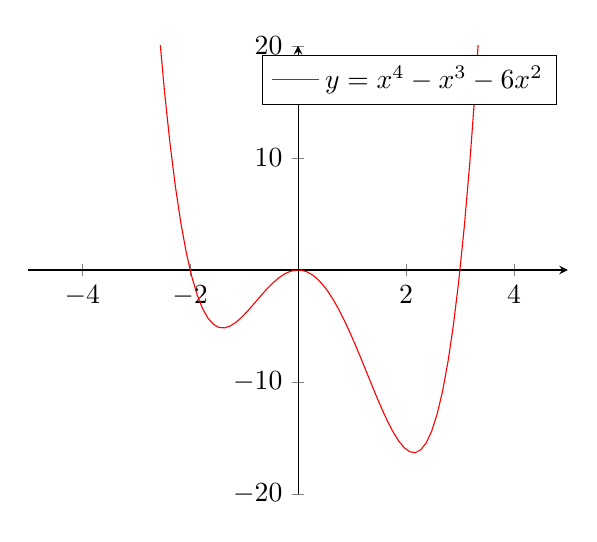
\begin{tikzpicture}
                \begin{axis}[
                    axis lines = center,
                    ymin = -20,
                    ymax = 20,
                    xmin = -5,
                    xmax = 5
                ]
                \addplot [
                    samples=100,
                    color=red
                ]
                {x^4-x^3-6*x^2};
                \addlegendentry{$y=x^4-x^3-6x^2$}
                \end{axis}
            \end{tikzpicture}
        \end{center}



    \subsection{Rational Root Test}
        Suppose we have a polynomial $P(x)$ with integer coefficients and a nonzero constant
        term, $a_n\not=0$. \\
        $P(x)=a_nx^n+a_{n-1}x^{n-1}+\dots+a_1x+a_0$ \\
        Then potential rational roots of $P(x)$ are of the form

        \begin{equation*}
            \frac{p}{q} = \frac{\pm\text{factors of }a_0}{\pm\text{factors of }a_n}
        \end{equation*}

        \noindent \color{blue} \textit{Example: Find the rational roots of
        $P(x)=3x^3-4x^2-17x+6$} \color{black} \\

        \noindent The leading coefficient is $a_n=3$ and constant term is $a_0=6$.
        We can determine the positive and negative factors of \\
        $a_0=6:\pm(1,2,3,6)$ \\
        $a_n=3:\pm(1,3)$ \\
        Then \\

        \begin{equation*}
            \frac{p}{q} = \frac{\pm(1,2,3,6)}{\pm(1,3)} = \pm 1, \pm\frac{1}{3}, \pm 2,
            \pm \frac{2}{3}, \pm 3, \pm \frac{3}{3}, \pm \frac{6}{1}, \pm \frac{6}{3}
        \end{equation*}

        \noindent Eliminating duplicate terms and simplifying, our root candidates are:

        \begin{equation*}
            \pm \frac{1}{3}, \pm\frac{2}{3}, \pm 1, \pm 2, \pm 3, \pm 6
        \end{equation*}

        \noindent We recall that if $a$ is a root of $P(x)$ then $P(a)=0$. Let's check our
        candidates now.

        % Table of candidates and if they are roots of function
        \begin{center}
            \begin{tabular}{|c|c|}
                \hline
                \textbf{$P(x)=3x^3-4x^2-17x+6$} & \textbf{Is it a root?} \\
                \hline
                $P(\frac{1}{3})=0$              & YES                    \\
                \hline
                $P(-\frac{1}{3})=\frac{100}{9}$ & No                     \\
                \hline
                $P(\frac{2}{3}=-\frac{56}{9}$   & No                     \\
                \hline
                $P(-\frac{2}{3})=\frac{44}{3}$  & No                     \\
                \hline
                $P(1)=-12$                      & No                     \\
                \hline
                $P(-1)=16$                      & No                     \\
                \hline
                $P(2)=-20$                      & No                     \\
                \hline
                $P(-2)=0$                       & YES                    \\
                \hline
                $P(3)=0$                        & YES                    \\
                \hline
                $P(-3)=-60$                     & No                     \\
                \hline
                $P(6)=408$                      & No                     \\
                \hline
                $P(-6)=-684$                    & No                     \\
                \hline
            \end{tabular}
        \end{center}